\documentclass[aspectratio=169,12pt]{beamer}

\usepackage[T1]{fontenc}
\usepackage[utf8]{inputenc}
\usepackage[ngerman]{babel}
\usepackage{lmodern}
\usepackage{graphicx}
\usepackage{xcolor}
\usepackage{tikz}
\usepackage{ragged2e}
\usepackage{hyperref}

\usetheme{default}

\definecolor{bg}{RGB}{12,12,12}
\definecolor{text}{RGB}{235,235,235}
\definecolor{muted}{RGB}{135,135,135}
\definecolor{accent}{RGB}{215,120,160}
\definecolor{ok}{RGB}{110,220,150}

\setbeamercolor{background canvas}{bg=bg}
\setbeamercolor{normal text}{fg=text,bg=bg}
\setbeamercolor{frametitle}{fg=text,bg=bg}
\setbeamercolor{title}{fg=text,bg=bg}
\setbeamercolor{item}{fg=accent}
\setbeamerfont{frametitle}{series=\bfseries,size=\large}
\setbeamerfont{title}{series=\bfseries}

\setbeamertemplate{navigation symbols}{}
\setbeamertemplate{footline}[frame number]

\setbeamertemplate{background}{%
\begin{tikzpicture}[remember picture,overlay]
  \fill[bg] (current page.south west) rectangle (current page.north east);
  \draw[white,opacity=0.025,line width=1pt]
    (current page.south west) -- (current page.north east);
\end{tikzpicture}%
}

\newcommand{\titleslide}[2]{%
\begin{frame}[plain,noframenumbering]
  \vfill
  \centering
  {\fontsize{42}{46}\selectfont\textbf{#1}}\\[0.6cm]
  {\Large\textcolor{muted}{#2}}
  \vfill
\end{frame}
}

\newcommand{\sectioncard}[2]{%
\begin{frame}[plain,noframenumbering]
  \vfill
  \centering
  {\Large\textcolor{muted}{#1}}\\[0.35cm]
  {\fontsize{34}{38}\selectfont\textbf{#2}}
  \vfill
\end{frame}
}

\newcommand{\teamcard}[1]{%
\begin{frame}[plain,noframenumbering]
  \vfill
  \centering
  {\Large\textcolor{muted}{Teamname}}\\[0.4cm]
  {\fontsize{34}{38}\selectfont\textbf{#1}}
  \vfill
\end{frame}
}

\newcommand{\textquestion}[4]{%
\begin{frame}{#1 --- #2 --- Frage #3}
  \vfill
  {\Large\justifying #4\par}
  \vfill
  \hfill{\small 1 Punkt}
\end{frame}
}

\newcommand{\textanswer}[4]{%
\begin{frame}{#1 --- #2 --- Antwort #3}
  \vfill
  \centering
  {\Large Die richtige Antwort ist:}\\[0.75cm]
  {\fontsize{28}{32}\selectfont\textbf{#4}}
  \vfill
\end{frame}
}

\newcommand{\mcquestionthree}[7]{%
\begin{frame}{#1 --- #2 --- Frage #3}
  {\Large\justifying #4\par}
  \vspace{0.7cm}
  \large
  \begin{itemize}
    \item[A:] #5
    \item[B:] #6
    \item[C:] #7
  \end{itemize}
  \vfill
  \hfill{\small 1 Punkt}
\end{frame}
}

\newcommand{\mcanswerthree}[8]{%
\begin{frame}{#1 --- #2 --- Antwort #3}
  {\Large\justifying #4\par}
  \vspace{0.7cm}
  \large
  \begin{itemize}
    \item[A:] #5
    \item[B:] #6
    \item[C:] #7
  \end{itemize}
  \vfill
  \textcolor{ok}{\Large\textbf{Richtig: #8}}
\end{frame}
}

\newcommand{\mcquestion}[8]{%
\begin{frame}{#1 --- #2 --- Frage #3}
  {\Large\justifying #4\par}
  \vspace{0.7cm}
  \large
  \begin{itemize}
    \item[A:] #5
    \item[B:] #6
    \item[C:] #7
    \item[D:] #8
  \end{itemize}
  \vfill
  \hfill{\small 1 Punkt}
\end{frame}
}

\newcommand{\mcanswer}[9]{%
\begin{frame}{#1 --- #2 --- Antwort #3}
  {\Large\justifying #4\par}
  \vspace{0.7cm}
  \large
  \begin{itemize}
    \item[A:] #5
    \item[B:] #6
    \item[C:] #7
    \item[D:] #8
  \end{itemize}
  \vfill
  \textcolor{ok}{\Large\textbf{Richtig: #9}}
\end{frame}
}

\newcommand{\imagequestion}[5]{%
\begin{frame}{#1 --- #2 --- Frage #3}
  \centering
  {\Large #4\par}
  \vspace{0.4cm}
  \includegraphics[width=0.83\textwidth,height=0.65\textheight,keepaspectratio]{#5}
  \vfill
  \hfill{\small 1 Punkt}
\end{frame}
}

\newcommand{\imageanswer}[6]{%
\begin{frame}{#1 --- #2 --- Antwort #3}
  \centering
  {\Large #4\par}
  \vspace{0.25cm}
  \includegraphics[width=0.58\textwidth,height=0.46\textheight,keepaspectratio]{#5}
  \vspace{0.35cm}

  {\Large\textcolor{ok}{\textbf{#6}}}
\end{frame}
}

\begin{document}

\titleslide{Kneipenquiz}{Bier \& Halbwissen}
\teamcard{Zum scheißenden Esel}

\begin{frame}{Regeln}
\Large
\begin{itemize}
  \item Keine Handys
  \item Keine Google-Skills
  \item Diskussionen erlaubt
  \item Viel Spaß
\end{itemize}
\end{frame}

\titleslide{Runde 1}{Brauereien, Wein, Trivia}

\sectioncard{Runde 1}{Brauereien}
\imagequestion{Runde 1}{Brauereien}{1}{Welche Brauerei ist das?}{assets/brauereien/frage1_augustiner.jpg}
\imagequestion{Runde 1}{Brauereien}{2}{Welche Brauerei ist das?}{assets/brauereien/frage2_bayreuther.jpg}
\imagequestion{Runde 1}{Brauereien}{3}{Welche Brauerei ist das?}{assets/brauereien/frage3_becks.jpg}
\imagequestion{Runde 1}{Brauereien}{4}{Welche Brauerei ist das?}{assets/brauereien/frage4_astra.jpg}
\imagequestion{Runde 1}{Brauereien}{5}{Welche Brauerei ist das?}{assets/brauereien/frage5_sudhang.jpg}

\sectioncard{Runde 1}{Wein}
\mcquestionthree{Runde 1}{Wein}{1}{Was bezeichnet man als Agraffe?}{Glasgefäß zum Abmessen}{Ausschenker}{Metalldraht zum Verschließen für Sekt oder Champagner}
\mcquestionthree{Runde 1}{Wein}{2}{Was ist ein Rosé-Wein?}{Weißwein und Rotweintrauben gemischt}{Weißwein mit Traubensaft}{Rotweintrauben weiß gekeltert}
\mcquestionthree{Runde 1}{Wein}{3}{Was bezeichnet \glqq Tempranillo\grqq?}{Anbaugebiet}{Traubensorte}{Weingut}
\mcquestionthree{Runde 1}{Wein}{4}{Welche Lagertemperatur ist für Rotwein richtig?}{21--22~°C}{12--16~°C}{18--19~°C}
\mcquestionthree{Runde 1}{Wein}{5}{Was bedeutet dekantieren?}{Weinflasche öffnen}{Weinverschnitt herstellen}{Wein Luft zuführen}

\sectioncard{Runde 1}{Trivia}
\textquestion{Runde 1}{Trivia}{1}{Was konnte man im ersten Automaten kaufen?}
\textquestion{Runde 1}{Trivia}{2}{Welcher Planet in unserem Sonnensystem hat den längsten Tag?}
\textquestion{Runde 1}{Trivia}{3}{Zu welcher Band gehören Robert Plant, Jimmy Page, John Paul Jones und John Bonham?}
\textquestion{Runde 1}{Trivia}{4}{In welchem Land wurden die Szenen auf Tatooine aus Star Wars gedreht?}
\textquestion{Runde 1}{Trivia}{5}{Wo wächst der giftigste bzw. gefährlichste Baum der Welt?}

\titleslide{Pause}{Getränke auffüllen}
\titleslide{Auflösung Runde 1}{Punkte ehrlich zählen}

\sectioncard{Auflösung Runde 1}{Brauereien}
\imageanswer{Runde 1}{Brauereien}{1}{Welche Brauerei ist das?}{assets/brauereien/frage1_augustiner.jpg}{Augustiner}
\imageanswer{Runde 1}{Brauereien}{2}{Welche Brauerei ist das?}{assets/brauereien/frage2_bayreuther.jpg}{Bayreuther}
\imageanswer{Runde 1}{Brauereien}{3}{Welche Brauerei ist das?}{assets/brauereien/frage3_becks.jpg}{Becks}
\imageanswer{Runde 1}{Brauereien}{4}{Welche Brauerei ist das?}{assets/brauereien/frage4_astra.jpg}{Astra}
\imageanswer{Runde 1}{Brauereien}{5}{Welche Brauerei ist das?}{assets/brauereien/frage5_sudhang.jpg}{Sudhang}

\sectioncard{Auflösung Runde 1}{Wein}
\mcanswerthree{Runde 1}{Wein}{1}{Was bezeichnet man als Agraffe?}{Glasgefäß zum Abmessen}{Ausschenker}{Metalldraht zum Verschließen für Sekt oder Champagner}{C}
\mcanswerthree{Runde 1}{Wein}{2}{Was ist ein Rosé-Wein?}{Weißwein und Rotweintrauben gemischt}{Weißwein mit Traubensaft}{Rotweintrauben weiß gekeltert}{C}
\mcanswerthree{Runde 1}{Wein}{3}{Was bezeichnet \glqq Tempranillo\grqq?}{Anbaugebiet}{Traubensorte}{Weingut}{B}
\mcanswerthree{Runde 1}{Wein}{4}{Welche Lagertemperatur ist für Rotwein richtig?}{21--22~°C}{12--16~°C}{18--19~°C}{C}
\mcanswerthree{Runde 1}{Wein}{5}{Was bedeutet dekantieren?}{Weinflasche öffnen}{Weinverschnitt herstellen}{Wein Luft zuführen}{C}

\sectioncard{Auflösung Runde 1}{Trivia}
\textanswer{Runde 1}{Trivia}{1}{Weihwasser}
\textanswer{Runde 1}{Trivia}{2}{Venus}
\textanswer{Runde 1}{Trivia}{3}{Led Zeppelin}
\textanswer{Runde 1}{Trivia}{4}{Tunesien}
\textanswer{Runde 1}{Trivia}{5}{USA / Karibik}

\titleslide{Runde 2}{Bilderrätsel, Ortskenntnisse, Gametrivia}

\sectioncard{Runde 2}{Bilderrätsel}
\imagequestion{Runde 2}{Bilderrätsel}{1}{Welche Augenzahl befindet sich am Ende des Weges oben?}{assets/bilderraetsel/frage1_wuerfel.png}
\imagequestion{Runde 2}{Bilderrätsel}{2}{Welche Vorlage ergänzt sinnvoll das Muster?}{assets/bilderraetsel/frage2_muster.png}
\imagequestion{Runde 2}{Bilderrätsel}{3}{Wie viele Dreiecke sind zu sehen?}{assets/bilderraetsel/frage3_dreiecke.png}
\imagequestion{Runde 2}{Bilderrätsel}{4}{What is the car's parking spot number?}{assets/bilderraetsel/frage4_parkplatz.png}
\imagequestion{Runde 2}{Bilderrätsel}{5}{Wie viele Züge mindestens?}{assets/bilderraetsel/frage5_hanoi.png}

\sectioncard{Runde 2}{Ortskenntnisse}
\textquestion{Runde 2}{Ortskenntnisse}{1}{In welcher Straße war das Vis A Vis?}
\mcquestionthree{Runde 2}{Ortskenntnisse}{2}{Bis wann war Amberg die Hauptstadt der Oberpfalz?}{1795}{1830}{1810}
\textquestion{Runde 2}{Ortskenntnisse}{3}{Wie hoch ist der Kirchturm der Basilika St. Martin?}
\mcquestionthree{Runde 2}{Ortskenntnisse}{4}{Wie war der Name der Braut der \glqq Amberger Hochzeit\grqq{} im Jahr 1474?}{Margerete}{Anna}{Elisabeth}
\textquestion{Runde 2}{Ortskenntnisse}{5}{Die ursprünglichen Farben der Figuren des Spiels \glqq Mensch ärgere dich nicht\grqq{} sind Rot, Grün, Gelb und \ldots?}

\sectioncard{Runde 2}{Gametrivia}
\imagequestion{Runde 2}{Gametrivia}{1}{Aus welchem Spiel stammt dieses Bild?}{assets/gametrivia/frage1_pokemon.jpg}
\imagequestion{Runde 2}{Gametrivia}{2}{Aus welchem Spiel stammt dieses Bild?}{assets/gametrivia/frage2_zelda.jpg}
\imagequestion{Runde 2}{Gametrivia}{3}{Aus welchem Spiel stammt dieses Bild?}{assets/gametrivia/frage3_gta_sa.jpg}
\imagequestion{Runde 2}{Gametrivia}{4}{Aus welchem Spiel stammt dieses Bild?}{assets/gametrivia/frage4_witcher.jpg}
\imagequestion{Runde 2}{Gametrivia}{5}{Aus welchem Spiel stammt dieses Bild?}{assets/gametrivia/frage5_mw2.jpg}

\titleslide{Pause}{Noch ein Bier?}
\titleslide{Auflösung Runde 2}{Zwischenstand}

\sectioncard{Auflösung Runde 2}{Bilderrätsel}
\imageanswer{Runde 2}{Bilderrätsel}{1}{Welche Augenzahl befindet sich am Ende des Weges oben?}{assets/bilderraetsel/frage1_wuerfel.png}{5}
\imageanswer{Runde 2}{Bilderrätsel}{2}{Welche Vorlage ergänzt sinnvoll das Muster?}{assets/bilderraetsel/frage2_muster.png}{B}
\imageanswer{Runde 2}{Bilderrätsel}{3}{Wie viele Dreiecke sind zu sehen?}{assets/bilderraetsel/frage3_dreiecke.png}{27}
\imageanswer{Runde 2}{Bilderrätsel}{4}{What is the car's parking spot number?}{assets/bilderraetsel/frage4_parkplatz.png}{87}
\imageanswer{Runde 2}{Bilderrätsel}{5}{Wie viele Züge mindestens?}{assets/bilderraetsel/frage5_hanoi.png}{7}

\sectioncard{Auflösung Runde 2}{Ortskenntnisse}
\textanswer{Runde 2}{Ortskenntnisse}{1}{Lederergasse}
\mcanswerthree{Runde 2}{Ortskenntnisse}{2}{Bis wann war Amberg die Hauptstadt der Oberpfalz?}{1795}{1830}{1810}{C}
\textanswer{Runde 2}{Ortskenntnisse}{3}{93~m (\(\pm\) 5\,\%)}
\mcanswerthree{Runde 2}{Ortskenntnisse}{4}{Wie war der Name der Braut der \glqq Amberger Hochzeit\grqq{} im Jahr 1474?}{Margerete}{Anna}{Elisabeth}{A}
\textanswer{Runde 2}{Ortskenntnisse}{5}{Schwarz}

\sectioncard{Auflösung Runde 2}{Gametrivia}
\imageanswer{Runde 2}{Gametrivia}{1}{Aus welchem Spiel stammt dieses Bild?}{assets/gametrivia/frage1_pokemon.jpg}{Pokémon}
\imageanswer{Runde 2}{Gametrivia}{2}{Aus welchem Spiel stammt dieses Bild?}{assets/gametrivia/frage2_zelda.jpg}{The Legend of Zelda}
\imageanswer{Runde 2}{Gametrivia}{3}{Aus welchem Spiel stammt dieses Bild?}{assets/gametrivia/frage3_gta_sa.jpg}{GTA San Andreas}
\imageanswer{Runde 2}{Gametrivia}{4}{Aus welchem Spiel stammt dieses Bild?}{assets/gametrivia/frage4_witcher.jpg}{The Witcher}
\imageanswer{Runde 2}{Gametrivia}{5}{Aus welchem Spiel stammt dieses Bild?}{assets/gametrivia/frage5_mw2.jpg}{Call of Duty: Modern Warfare 2}

\titleslide{Runde 3}{Meme-Quiz, Geographie, Tierfragen}

\sectioncard{Runde 3}{Meme-Quiz}
\imagequestion{Runde 3}{Meme-Quiz}{1}{Welches Meme ist gemeint?}{assets/memes/frage1_spitzkopf.png}
\imagequestion{Runde 3}{Meme-Quiz}{2}{Welches Meme ist gemeint?}{assets/memes/frage2_kranplaetze.png}
\imagequestion{Runde 3}{Meme-Quiz}{3}{Welches Meme ist gemeint?}{assets/memes/frage3_perfect.png}
\imagequestion{Runde 3}{Meme-Quiz}{4}{Welches Meme ist gemeint?}{assets/memes/frage4_67.png}
\imagequestion{Runde 3}{Meme-Quiz}{5}{Welches Meme ist gemeint?}{assets/memes/frage5_fantasie.png}

\sectioncard{Runde 3}{Geographie}
\mcquestion{Runde 3}{Geographie}{1}{Welche dieser Hauptstädte liegt am nördlichsten?}{Oslo}{Helsinki}{Reykjavik}{Stockholm}
\mcquestion{Runde 3}{Geographie}{2}{Welche deutsche Stadt hat die meisten Brücken?}{Berlin}{Hamburg}{Leipzig}{Köln}
\mcquestion{Runde 3}{Geographie}{3}{In welchem Land gibt es die meisten Pyramiden?}{Sudan}{Ägypten}{Äthiopien}{Oman}
\mcquestion{Runde 3}{Geographie}{4}{Welches Bundesland grenzt an die meisten Bundesländer?}{Hessen}{Thüringen}{Sachsen-Anhalt}{Niedersachsen}
\mcquestion{Runde 3}{Geographie}{5}{Welche Stadt ist auch bekannt als die \glqq Stadt der sieben Hügel\grqq?}{Istanbul}{Lissabon}{Rom}{Edinburgh}

\sectioncard{Runde 3}{Tierfragen}
\mcquestion{Runde 3}{Tierfragen}{1}{Welches Tier hat den stärksten Biss der Welt?}{Weißer Hai}{Alligator-Schnappschildkröte}{Nilkrokodil}{Hyäne}
\mcquestion{Runde 3}{Tierfragen}{2}{Welches Tier ist KEIN Säugetier?}{Delfin}{Fledermaus}{Pinguin}{Wal}
\mcquestion{Runde 3}{Tierfragen}{3}{Welche besonderen Zellen helfen dem Chamäleon dabei, die Farbe zu wechseln?}{Melanozyten}{Chromatophoren}{Neuronen}{Keratinozyten}
\mcquestion{Runde 3}{Tierfragen}{4}{Welches Tier kann am längsten die Luft anhalten?}{Delfin}{Pinguin}{Pottwal}{Seelöwe}
\mcquestion{Runde 3}{Tierfragen}{5}{Welches Säugetier lebt fast wie ein Insektenstaat mit einer Königin?}{Erdmännchen}{Präriehund}{Hamster}{Nacktmull}

\titleslide{Letzte Auswertung}{Finale Punkte zählen}
\titleslide{Auflösung Runde 3}{Finale}

\sectioncard{Auflösung Runde 3}{Meme-Quiz}
\imageanswer{Runde 3}{Meme-Quiz}{1}{Welches Meme ist gemeint?}{assets/memes/frage1_spitzkopf.png}{Du nennst mich Spitzkopf?}
\imageanswer{Runde 3}{Meme-Quiz}{2}{Welches Meme ist gemeint?}{assets/memes/frage2_kranplaetze.png}{Kranplätze müssen verdichtet sein!}
\imageanswer{Runde 3}{Meme-Quiz}{3}{Welches Meme ist gemeint?}{assets/memes/frage3_perfect.png}{Perfect! / It was perfect!}
\imageanswer{Runde 3}{Meme-Quiz}{4}{Welches Meme ist gemeint?}{assets/memes/frage4_67.png}{67}
\imageanswer{Runde 3}{Meme-Quiz}{5}{Welches Meme ist gemeint?}{assets/memes/frage5_fantasie.png}{Mit einer Menge Fantasie}

\sectioncard{Auflösung Runde 3}{Geographie}
\mcanswer{Runde 3}{Geographie}{1}{Welche dieser Hauptstädte liegt am nördlichsten?}{Oslo}{Helsinki}{Reykjavik}{Stockholm}{C}
\mcanswer{Runde 3}{Geographie}{2}{Welche deutsche Stadt hat die meisten Brücken?}{Berlin}{Hamburg}{Leipzig}{Köln}{B}
\mcanswer{Runde 3}{Geographie}{3}{In welchem Land gibt es die meisten Pyramiden?}{Sudan}{Ägypten}{Äthiopien}{Oman}{A}
\mcanswer{Runde 3}{Geographie}{4}{Welches Bundesland grenzt an die meisten Bundesländer?}{Hessen}{Thüringen}{Sachsen-Anhalt}{Niedersachsen}{D}
\mcanswer{Runde 3}{Geographie}{5}{Welche Stadt ist auch bekannt als die \glqq Stadt der sieben Hügel\grqq?}{Istanbul}{Lissabon}{Rom}{Edinburgh}{C}

\sectioncard{Auflösung Runde 3}{Tierfragen}
\mcanswer{Runde 3}{Tierfragen}{1}{Welches Tier hat den stärksten Biss der Welt?}{Weißer Hai}{Alligator-Schnappschildkröte}{Nilkrokodil}{Hyäne}{C}
\mcanswer{Runde 3}{Tierfragen}{2}{Welches Tier ist KEIN Säugetier?}{Delfin}{Fledermaus}{Pinguin}{Wal}{C}
\mcanswer{Runde 3}{Tierfragen}{3}{Welche besonderen Zellen helfen dem Chamäleon dabei, die Farbe zu wechseln?}{Melanozyten}{Chromatophoren}{Neuronen}{Keratinozyten}{B}
\mcanswer{Runde 3}{Tierfragen}{4}{Welches Tier kann am längsten die Luft anhalten?}{Delfin}{Pinguin}{Pottwal}{Seelöwe}{C}
\mcanswer{Runde 3}{Tierfragen}{5}{Welches Säugetier lebt fast wie ein Insektenstaat mit einer Königin?}{Erdmännchen}{Präriehund}{Hamster}{Nacktmull}{D}

\titleslide{Danke fürs Mitspielen}{Gewinnerteam: \underline{\hspace{5cm}}}

\begin{frame}[plain,noframenumbering]
  \centering
  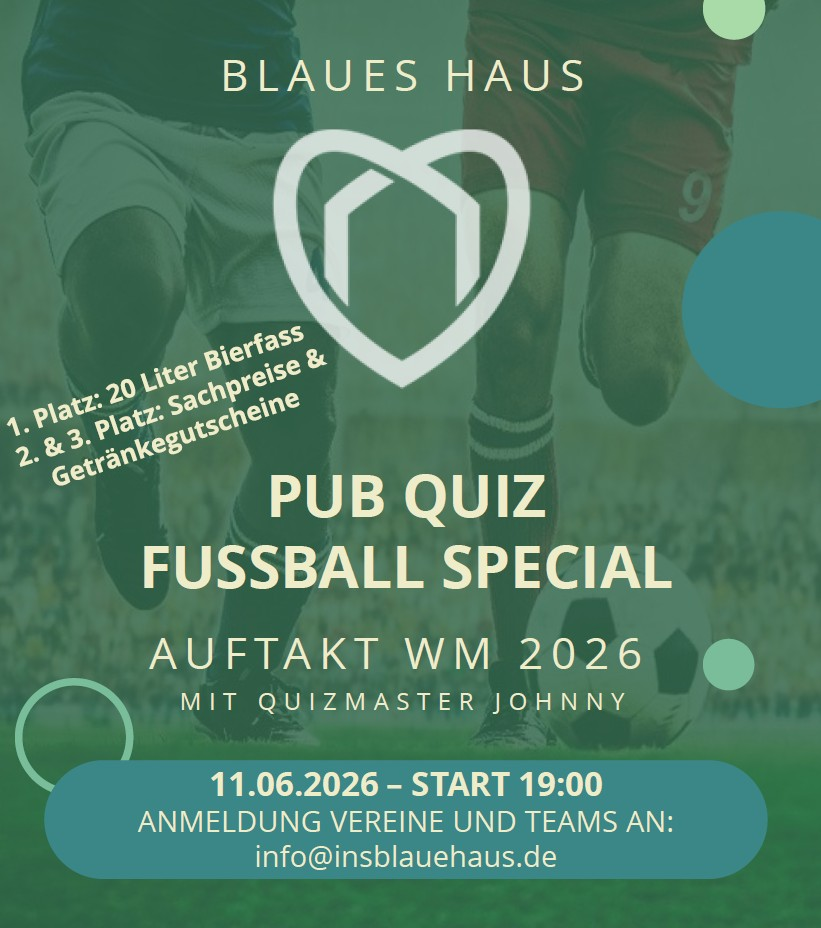
\includegraphics[width=0.92\textwidth,height=0.92\textheight,keepaspectratio]{assets/pubquiz_fussball_special.png}
\end{frame}

\end{document}
